\documentclass[a4paper]{article}
\usepackage[utf8]{inputenc}
\usepackage[frenchb]{babel}
\usepackage[T1]{fontenc}
\usepackage{graphicx}
\usepackage{ifpdf}
\usepackage{hyperref}
\usepackage{amsmath}
\usepackage{slashbox}

\title{Processeu \textsc{Nono} 1et 2}
\author{Cédric \textsc{Bois} \and Benjamin \textsc{Sientzoff}}
\date{\today}
\ifpdf
\hypersetup{
    pdfauthor={Cédric Bois, Benjamin Sientzoff},
    pdftitle={Réalisation processeur Nono-1 et Nono-2},
}
\fi
\begin{document}
	% page de garde avec sommaire
	\maketitle
	\newpage
	% sommaire
	\tableofcontents
	\newpage % passer à la page suivante
	
	\section*{Introduction}

		\paragraph{}{
		Dans le cadre du cours intitulé \textit{Architecture des ordinateurs}, nous devons recréer
		un processeur Nono-1. Par la suite, ce processeur sera modifier pour devenir Nono-2. Ce 
		rapport retrace comment nous avons réalisé ces processeurs MIPS.
		}
		
		\paragraph{}{
		Les circuits électroniques présentés sont produits avec le logiciel \textit{Logisim}. Ces
		circuits et les différents fichiers permettant notamment de programmer le processeur sont 
		fournis avec la version numérique de ce rapport. Les images RAM peuvent être directement 
		chargées dans la RAM des processeurs Nono. Ces images correspondent aux programmes 
		compilés pour ces architectures et peuvent être exécutés directement dans \textit{Logisim}.
		}
		
		\paragraph{}{
		Dans une première partie, nous présentons les différents sous-circuits composants le 
		processeur Nono-1. Une seconde partie présente sont fonctionnement global et les 
		modifications apportées à Nono-1 pour implémenter les fonctions de Nono-2.
		}
	
	\newpage
	%\section{Réalisation de Nono-1}
	
		\section{Opcode des instructions}
			
			\paragraph{}{
			Nono-1 et Non-2 sont des processeurs utilisant l'assembleur MIPS. Les 
			instructions disponibles sur Nono-1 sont présentés au tableau de la figure
			\ref{tab_opcode}. On remarque que les instructions reconnues sont relativement
			restreintes. Ces instructions sont de trois formats différents comme on peut
			le voir à la figure \ref{format_inst}\footnote{Tiré du sujet du projet rédigé par M. Frédéric \textsc{Goualard}}.
			}
			
			\begin{figure}[!ht]
			\centering
			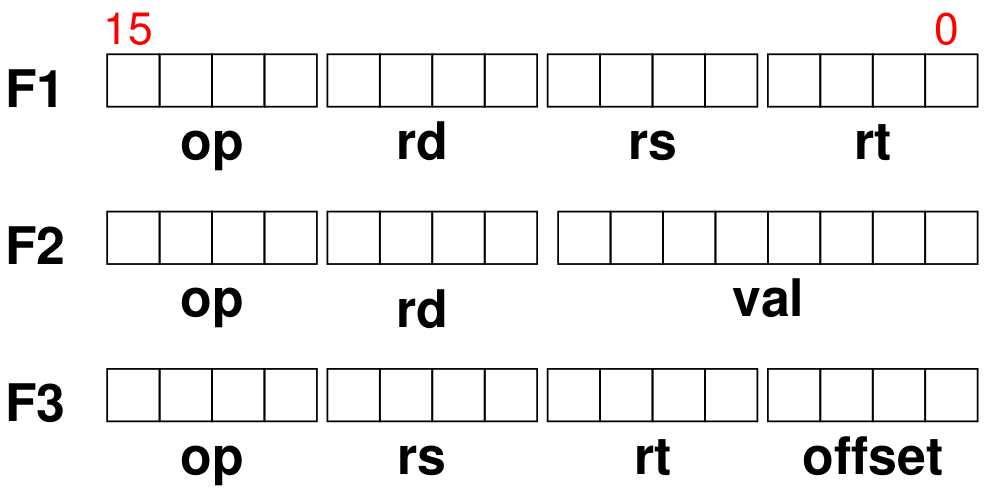
\includegraphics[scale=0.2]{formats_instructions.png}
			\caption{\label{format_inst} Formats des instructions}
			\end{figure}
			
				\subparagraph{Le Format F1}{
				Le format F1 est composé de quatre paquets de bits.
				Le premier est sur quatre bits, il correspond au code de l'instruction,
				et c'est le cas pour tous les formats d'instructions.
				Les trois paquets suivants, sur quatre bits. Ce format est utilisé typiquement
				pour des opérations faisant intervenir trois registres. Le premier correspond
				à la destination du résultat et les deux suivants aux registres contenant les
				opérantes.
				}
				\subparagraph{Le Format F2}{
				Le format F2 est composé de trois paquets de bits.
				Le premier est sur quatre bits, il correspond au code de l'instruction.
				Les 4 bits suivants correspondent à un nom de registre et les 8 derniers
				à une valeur immédiate. Ce format est typiquement utilisé pour l'instruction
				\textit{li}.
				}
				\subparagraph{Le Format F3}{
				Le format F3 peut être divisé en quatre parties. C'est le format utilisé
				pour les sauts. Les quatre bits correspondent à l'opcode de l'instruction.
				Le paquet des quatre bits et le suivant constitué des quatre autres bits
				suivant correspondent à des noms de registres. Enfin les derniers bits (au
				nombre de quatre) correspondent à un offset. Pour les sauts, cela correspond
				à l'adresse de l'étiquette où effectuer le saut. 
				}
			
			\begin{figure}
			\centering
			\begin{tabular}{|p{4cm}|c|c|c|c|}
				\hline Instruction et paramètres & Format & Opcode  \\ 
				\hline \texttt{add r$_{d}$, r$_{s}$, r$_{t}$} & F$_{1}$ & \texttt{1000} \\ 
				\hline \texttt{sub r$_{d}$, r$_{s}$, r$_{t}$} & F$_{1}$ & \texttt{1001}  \\ 
				\hline \texttt{or r$_{d}$, r$_{s}$, r$_{t}$} & F$_{1}$ & \texttt{1010}  \\ 
				\hline \texttt{and r$_{d}$, r$_{s}$, r$_{t}$} & F$_{1}$ & \texttt{1011}  \\ 
				\hline \texttt{not r$_{d}$, r$_{s}$} & F$_{1}$ & \texttt{1100} \\ 
				\hline \texttt{shl r$_{d}$, r$_{s}$, r$_{t}$} & F$_{1}$ & \texttt{1101} \\ 
				\hline \texttt{shr$_{d}$, r$_{s}$, r$_{t}$} & F$_{1}$ & \texttt{1110} \\ 
				\hline \texttt{li r$_{d}$, $val$} & F$_{2}$ & \texttt{1111} \\ 
				\hline \texttt{halt} & F$_{1}$ & \texttt{0000} \\ 
				\hline \texttt{b \textit{offset}} & F$_{3}$ & \texttt{0001} \\
				\hline \texttt{beq r$_{s}$, r$_{t}$, \textit{offset}} & F$_{3}$ & \texttt{0010} \\ 
				\hline \texttt{bne r$_{s}$, r$_{t}$,\textit{offset}} & F$_{3}$ & \texttt{0011} \\ 
				\hline \texttt{bge r$_{s}$, r$_{t}$, \textit{offset}} & F$_{3}$ & \texttt{0100} \\ 
				\hline \texttt{ble r$_{s}$, r$_{t}$, \textit{offset}} & F$_{3}$ & \texttt{0101} \\ 
				\hline \texttt{bgt r$_{s}$, r$_{t}$, \textit{offset}} & F$_{3}$ & \texttt{0110} \\ 
				\hline \texttt{blt r$_{s}$, r$_{t}$, \textit{offset}} & F$_{3}$ & \texttt{0111} \\ 
				\hline 
				\end{tabular}
			\caption{
				\label{tab_opcode}
				\textit{Opcode} des différentes instruction du processeur \textsc{Nono 1}
			}
			\end{figure}
			
			\paragraph{}{
			Le choix des opcodes n'a pas était fait au hasard. En effet, en regardant le nombre
			d'instructions pour les sauts et le nombre d'opérations faisant appellent à l'unité
			arithmétique et logique du processeur, on s’aperçoit qu'ils peuvent être divisé 
			en deux 	groupes. On a donc regroupés les opcodes en trois groupes. Le premier 
			correspond aux opcodes qui commence par un $1$, ce sont les instructions qui font 
			appel à l'UAL. Le second groupe, les opcodes commencent par un $0$, correspondent 
			aux sauts. Enfin le dernier groupe est composé des autres instructions. Citons
			notamment les opcodes $0000$ et $1111$. Le tableau des instructions, leur format et
			les opcodes correspondants est présenté à la figure \ref{tab_opcode}.
			}
			
			\paragraph{}{
			Maintenant que nous avons définit nos opcodes, il est temps de concevoir les circuits
			électroniques composants le processeur \textsc{Nono 1}. Commençons par l'Unité 
			Arithmétique et Logique.
			}
	
		\section{L' unité arithmétique et logique}
			\paragraph{}{
	intro, explications
}

\begin{figure}
	\centering
	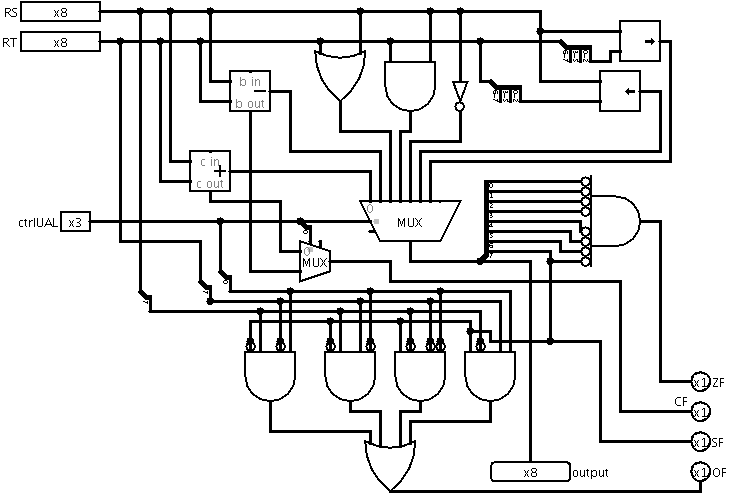
\includegraphics[scale=0.5,origin=c]{circuits/UAL.png}
	\label{ual_circ}
	\caption{Sch\'{e}ma \'{e}lectronique de l'Unit\'{e} Arithm\'{e}tique et Logique}
\end{figure}
			
		\section{Le contrôleur de saut}
			\paragraph{}{
	Le second circuit éléectronique composant le processeur est
	le contrôleur de saut. Son rôle est de mettre à jour \textit{PC}
	en fonction du résultat de l'opération que vient d'effectuer
	l'UAL pour le cycle suivant. Le saut est déterminé en fonction
	des indicateurs que le circuit à en entrée, c'est-à-dire 
	\textit{SF} et \textit{ZF}. Pour celà, on fait un tableau de
	Karnaugh, à la figure \ref{karnaugh_ctrl_saut}.
}

\begin{figure}
	\centering
	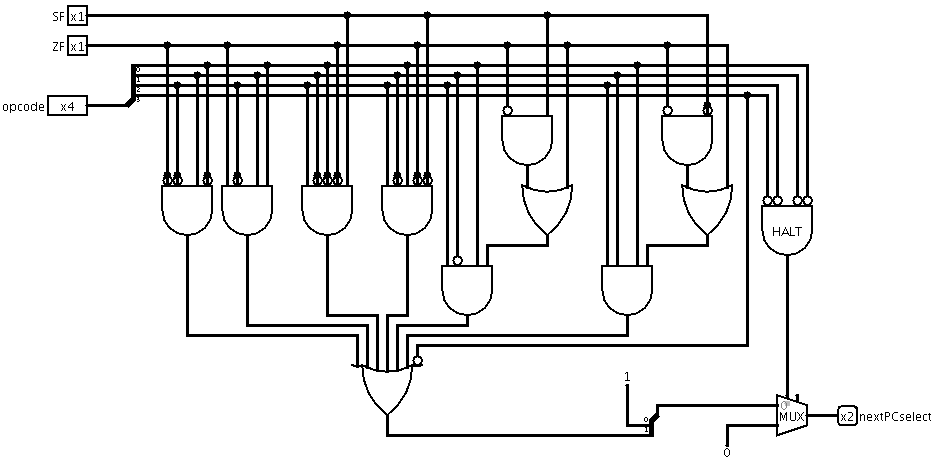
\includegraphics[scale=0.4,origin=c]{circuits/control_saut.png}
	\label{control_saut_circ}
	\caption{Sch\'{e}ma \'{e}lectronique du contr\^{o}leur de sauts}
\end{figure}

\begin{figure}
	\centering
	\begin{tabular}{|c|c|c|c|c|c|}
		\hline 
		O2 & O1 & O0 & ZF & SF & C1 \\ 
		\hline 
		$0$ & $0$ & $1$ & $\times$ & $\times$ & $0$ \\ 
		\hline 
		$0$ & $1$ & $0$ & $0$ & $\times$ & $1$ \\ 
		\hline 
		$0$ & $1$ & $0$ & $0$ & $\times$ & $0$ \\ 
		\hline 
		$0$ & $1$ & $1$ & $1$ & $\times$ & $0$ \\ 
		\hline 
		$0$ & $1$ & $1$ & $1$ & $\times$ & $1$ \\ 
		\hline 
		$1$ & $0$ & $0$ & $0$ & $0$ & $0$ \\ 
		\hline 
		$1$ & $0$ & $0$ & $0$ & $1$ & $1$ \\ 
		\hline 
		$1$ & $0$ & $0$ & $1$ & $0$ & $0$ \\ 
		\hline 
		$1$ & $0$ & $0$ & $1$ & $1$ & $0$ \\ 
		\hline 
		$1$ & $0$ & $1$ & $0$ & $0$ & $1$ \\ 
		\hline 
		$1$ & $0$ & $1$ & $0$ & $1$ & $0$ \\ 
		\hline 
		$1$ & $0$ & $1$ & $1$ & $0$ & $0$ \\ 
		\hline 
		$1$ & $0$ & $1$ & $1$ & $1$ & $0$ \\ 
		\hline 
		$1$ & $1$ & $0$ & $0$ & $0$ & $0$ \\ 
		\hline 
		$1$ & $1$ & $0$ & $0$ & $1$ & $1$ \\ 
		\hline 
		$1$ & $1$ & $0$ & $1$ & $0$ & $1$ \\ 
		\hline 
		$1$ & $1$ & $0$ & $1$ & $1$ & $1$ \\ 
		\hline 
		$1$ & $1$ & $1$ & $0$ & $0$ & $1$ \\ 
		\hline 
		$1$ & $1$ & $1$ & $0$ & $1$ & $0$ \\ 
		\hline 
		$1$ & $1$ & $1$ & $1$ & $0$ & $1$ \\ 
		\hline 
		$1$ & $1$ & $1$ & $1$ & $1$ & $1$ \\ 
		\hline 
	\end{tabular} 
	\label{karnaugh_ctrl_saut}
	\caption{Tableau de Karnaugh du contrôleur de saut}
\end{figure}

\paragraph{}{
	Le schéma électronique du contrôleur de saut est à la figure
	\ref{control_saut_circ}. 
}
			
		\section{Le décodeur d'instructions}
			\paragraph{}{
	Le décodeur d'instructions permet de déterminer quel opération va effectuer
	le processeur pour le cycle à venir. C'est lui qui lit les opcodes déterminés
	précédemment.
}
	\subparagraph{Gestion des sauts}{
		Lorsque le décodeur de sauts lis une instruction de type \textit{b},
		il se contente d'appeler l'Unité Arithmétique et logique pour faire
		une soustraction. Il arme également la sortie \textit{isJMP}.
	}

\begin{figure}
	\centering
	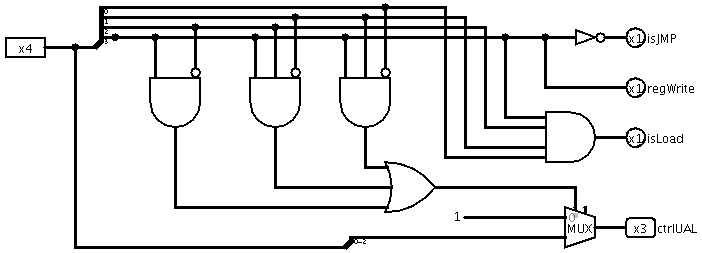
\includegraphics[scale=0.4,origin=c]{circuits/deco_instru.png}
	\caption{
		\label{decod_inst_circ}
		Sch\'{e}ma \'{e}lectronique pour le d\'{e}codeur d'instructions
		}
\end{figure}

\paragraph{}{
	Le schéma électronique du décodeur d'instructions est présenté à la figure
	\ref{decod_inst_circ}. La partie qui décode le signal \textit{ctrlUAL} 
	correspond au tableau de \textsc{Karnaugh} de la figure 
	\ref{decod_ctrlual_karnaugh} duquel on extrait l'équation suivante :
	\begin{equation}
		ctralUAL = b_{3} . \neg b_{2} + b_{3} . b_{2} \neg b_{1}  + b_{3} . b_{1} \neg b_{0}
		\label{equation_ual}
	\end{equation}
	Cette équation nous permet alors de réaliser le circuit électronique 
	décodant \textit{ctrlAUL}.
}

\begin{figure}
	\begin{center}
	\centering
	\begin{tabular}{|c|c|c|c|c|}
		\hline
		\backslashbox{$b_{3}b_{2}$}{$b_{1}b_{0}$} & $00$ & $01$ & $11$ & $10$ \\ 
		\hline 
		$00$ & $0$ & $0$ & $0$ & $0$ \\ 
		\hline 
		$01$ & $0$ & $0$ & $0$ & $0$ \\ 
		\hline 
		$11$ & $1$ & $1$ & $0$ & $1$ \\ 
		\hline 
		$10$ & $1$ & $1$ & $1$ & $1$ \\ 
		\hline 
	\end{tabular} 
	\end{center}
	\caption{
		\label{decod_ctrlual_karnaugh}
		Tableau de \textsc{Karnaugh} pour le décodage d'instructions.
	}
\end{figure}
			
		\section{La sélection des registres}
			\paragraph{}{
	Le sélecteur de registres permet de déterminer le registre
	dans lequel on va lire ou écrire un octet. Son circuit électronique
	est présenté à la figure \ref{selec_reg_circ}.
	Sont fonctionnement est relativement simple, on ne s’attardera donc
	pas dessus.
}

\begin{figure}
	\centering
	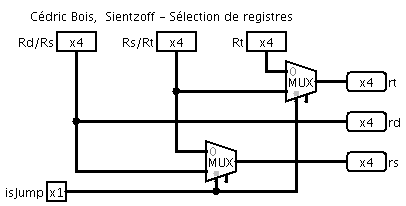
\includegraphics[scale=0.8,origin=c]{circuits/selec_reg.png}
	\caption{
		\label{selec_reg_circ}
		Sch\'{e}ma \'{e}lectronique pour la s\'{e}lection de registres
	}
\end{figure}

\paragraph{}{
	Maintenant que nous sommes en capacité de choisir un registre
	et l'opération qu'on souhaite y faire, réalisons le banc de
	registres.
}
			
		\section{Le banc de registres}
			\paragraph{}{
	Le banc de registres constitue la mémoire du processeur. Il possède
	16 registres d'un octet. Un tel circuit	est composé de bascules
	D en cascade. Il y en a une pour chaque registre. Il est à la figure
	\ref{banc_reg_circ}. \newline
	L'écriture d'un registre est possible uniquement lorsque \textit{regWrite}
	est à vrai.
}

\begin{figure}
	\centering
	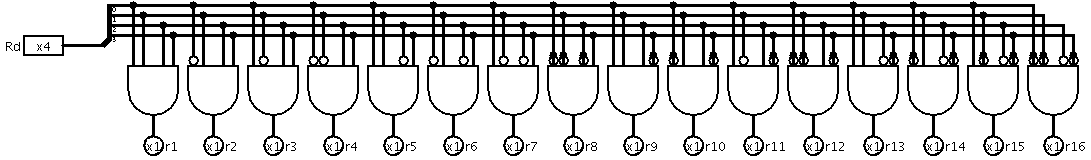
\includegraphics[scale=0.4,angle=90,origin=c]{circuits/banc_reg.png}
	\caption{
		\label{banc_reg_circ}
		Sch\'{e}ma \'{e}lectronique pour le banc de registres
	}
\end{figure}

	\subparagraph{Sélecteur de registres}{
		Attention, le sélecteur à la figure \ref{banc_reg_selec_circ}, n'est
		pas le même que le sélecteur de registres présenté en amont.
		Celui-ci est spécifique au banc de registres. C'est le circuit
		\textit{BC selec Reg} sur le schéma à la figure \ref{banc_reg_circ}.
	}

\begin{figure}
	\centering
	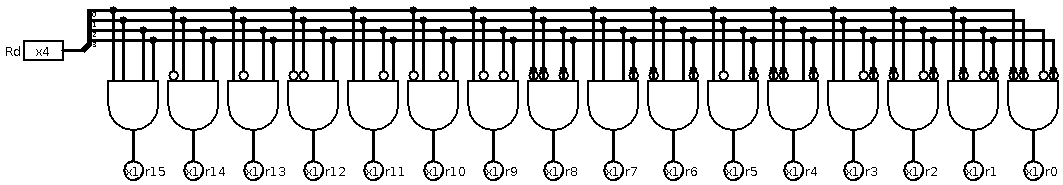
\includegraphics[scale=0.3,origin=c]{circuits/banc_reg_selec.png}
	\caption{
		\label{banc_reg_selec_circ}
		Sch\'{e}ma \'{e}lectronique pour le sélecteur du banc de registres
	}
\end{figure}
	
	\newpage	
	%\section{Processeurs Nono-1 et Nono-2}
		\section{Nono-1}
		\section{Nono-2}
	

	
	
	\newpage
	\section*{Conclusion}
		\paragraph{}{je conclu}
		
	\newpage
	\listoffigures
		
\end{document}
